\documentclass[twocolumn]{article}
\usepackage[utf8]{inputenc}
\usepackage{amsmath}
\usepackage{natbib}
\usepackage{graphicx}
\usepackage{astrojournals}
\bibliographystyle{apj}
\usepackage[spanish, es-minimal, english]{babel}
\usepackage[vmargin=0.8in, hmargin=1.00in]{geometry}
%\usepackage[demo]{graphicx}
%\usepackage{floatrow}
%\caption{caption text}
\usepackage{sidecap}
\usepackage{hyperref}
\usepackage{cleveref}
\crefname{section}{§}{§§}
\Crefname{section}{§}{§§}


\setlength{\fboxsep}{0pt}%
\newlength\figwidth
\setlength\figwidth{0.48\textwidth}
\setlength\tabcolsep{0pt}
\newcommand\raiselabel[1]{\raisebox{0.39\figwidth}[-0.39\figwidth]{#1}}
%\renewcommand{\baselinestretch}{1.3}
\newcommand{\gt}{>}
\newcommand\U[1]{\ensuremath{\mathrm{#1}}}
\newcommand\msol{M_\odot}
\newcommand\msolagno{M_\odot\,\U{yr^{-1}}}

%\newcommand\U[1]{\ensuremath{\mathrm{#1}}}
\newcommand\K{\U{K}}
\newcommand\cm{\U{cm}}
\newcommand\AU{\U{AU}}
\newcommand\g{\U{g}}

\newcommand\acre{\ensuremath{_{\mathrm{acre}}}}
\newcommand\eff{\ensuremath{_{\mathrm{eff}}}}
\newcommand\Ext{\ensuremath{_{\mathrm{Ext}}}}
\newcommand\Int{\ensuremath{_{\mathrm{Int}}}}

\newcommand\ha{\ensuremath{\mathrm{H\alpha}}}
\newcommand\oiii{\ensuremath{\mathrm{[O\,III]}}}
\newcommand\A{\ensuremath{\text{\AA{}}}}

%% Commands for the postage stamp images
\setlength{\fboxsep}{0pt}%
%\newlength\figwidth
\setlength\figwidth{0.46\textwidth}
\newlength\figstampcolsep
\setlength\figstampcolsep{5pt}
\newcommand\BowshockFig[1]{
  \includegraphics[width=\figwidth, clip, trim=10 10 10 10]
  {#1}
}
\newcommand\BowshockFigImg[1]{
  \includegraphics[width=0.5\figwidth, clip, trim=350 50 350 50]                 %Images
  {#1}
}

\newcommand\BowshockFigImag[1]{
  \includegraphics[width=0.9\figwidth, clip, trim=20 20 10 10]                 %Images
  {#1}
}
%\newcommand\raiselabel[1]{\raisebox{0.9\figwidth}[-0.5\figwidth]{#1}}


\title{Discovery of a new high-ionization planetary nebula in LAMOST}

\author{Luis A. Gutiérrez Soto     
}

\begin{document}
\maketitle

\section{Introduction}
\label{sec:intro}

Planetary nebulae (PNe) represent the last stage of evolution of low- and intermediate-mass stars
(0.8$\msol$ - 8.0$\msol$). The PNe phase begin when gas is ejected from the red giant stars late
in their lives and subsequently this gas is ionized by the radiation field coming from the remnant
star resulted. An emission nebula expands, a glowing shell of ionized gas until lost in the
interstellar medium. Then the dying star core becomes a white dwarf.

The number of the PNe discovered in the galaxy is relatively low (\(\sim 3,500\)). However,
this current number of PNe represents only about 15-30\% of the estimated
total of Galactic PNe (\citealp{Frew:2008}; \citealp{Jacoby:2010}) showing that a small fraction
of the PNe have been cataloged \citep{Frew:2017}. If this is true, there will be a much larger
number of PNe in the Galaxy than if a special condition
is required. The models of \citet{Moe:2006}, for
example, predict that there are 46 000 ± 22 000 for the general case,
but only ∼6600 (De Marco & Moe 2005) if
close binaries (e.g. common-envelope phase) are required.
Miszalski et al. (2009) confirm earlier estimates that the
binary fraction of PN central stars is only 10–20\% of all
PNe, and thus, binarity is not likely to be a major factor in
the formation process. If true, there should be many PNe
waiting to be found in the Galaxy. This mean that the search for planetary nebulae
becoming a important task, that eavery time is more dificult, due to many of
the undiscovered PNe are probably
the more distant and then the more the weak. And because many of them, probably, are located
in nuvens of dust. And note that planetary nebulae only last for about 5,000-
25,000 yr \citep{Badenes:2015}, making them a very short-lived part of the stellar life cycle.
But is import to discovery new planetary nebula? the answer could be very obvious and is
related with the idea that PNe provide vital clues for the understanding late-stage stellar
evolution and Galactic chemical enrichment. Their strong emission lines allow the determination
of abundances, expansion and radial velocities, and
CSPN temperatures. The PN phase
enriches the ISM with nitrogen, carbon, helium, and dust,
important components in the formation of future generations
of stars. PNe yield information on the nuclear
burning, dredge up, and mass loss in the stellar progenitor
(see \citealp{Kwitter:2022} for an excellent recent PN
review). Thus, we need to know the number of PNe in
the Galaxy in order to develop accurate models of the
chemical enrichment rates since the initial burst of Type II
supernovae when the Galaxy was young.

PN studies have been hampered by three problems:
(i) the previous lack of accurate distances to most Galactic
PNe; (ii) obtaining representative PNe samples of the true
population diversity \citep{Parker:2022}, and (iii) their unknown
progenitor masses. The first problem has prospects of
resolution via accurate Gaia CSPN distances, though many
CSPNe remain too distant and faint for Gaia DR3 and correct
CSPN identification remains an issue for some (Parker et al.
2022). The second problem is being addressed by deep, narrow-band,
wide-field surveys, e.g., \citet{Parker:2005},
\citet{Drew:2005}, and Drew et al. (2014). For the third problem
of progenitor masses, these can only
be accurately determined for PNe in Galactic globular and
open clusters (OCs). These allow precise distance determinations
from color–magnitude diagrams (CMD) and Gaia \citep{Fragkou:2022}.

\section{Surveys}
\label{sec:surveys}

\subsection{GAIA EDR3}
\label{sec:gaia}

\subsection{Pan-STARRS DR1}
\label{sec:PS1}

\subsection{LAMOST}
\label{sec:lamost}

The Large Sky Area Multi-Object Fiber Spectroscopic Telescope
(LAMOST, also named Guoshoujing Telescope) is a
telescope dedicated for spectroscopic sky survey.
There are 4000 fibers within a diameter of 1.75 meters (corresponding
to 5$^{\circ}$ in the sky) at the focal surface \citep{Cui:2012}.
The Low-Resolution Spectroscopic Survey (LRS) of LAMOST
began in October 2011, with a spectral resolving power ($R = \lambda/\Delta\lambda$)
of about 1800 and a wavelength coverage of
3700-9100~\AA \citep{Zhao:2012}. The first year observation was
for the pilot survey (Luo et al. 2012; Zhao et al. 2012),
and the regular survey began in September 2012


\section{Methodology}
\label{sec:metho}

At the beginning the idea was to identify for new planetary nebula in GAIA.
I started to constructed possibles color-color diagrams to separate PNe from
other emission lines objects and stars using GAIA only. The separation was not
good because PNe, normal stars and other emission line stars like CVs occupy the same region
in the diagram. Then, I decided to move to Pan-STARRS and combining the two
surveys Pan-STARRS and GAIA. I found one color diagram that isolate the PNe
with, I suppose, strong \ha{} emission line. By using the \((G - r)\) versus \((G_{BP} - G_{RP})\)
color-color is possible to separate those PNe excess in the in the $r$-broad-band
filter as is possible to see in the Fig~\ref{fig:gaia-ps}. Fig~\ref{fig:gaia-ps}
shows that the many of the PNe have value in the color \(G - r\) = 0, however several
PNe cover the interval in this same color between 0 and 8, and span between -1 and 5.
The orange contours represent other emission line objects that includes CV, SySt,
YSOs, AeBe stars and SNRs. The contours becoming white at the outside indicating
that the number of objects decrease significantly. And the blue contours signify
stars from \citet{Smart:2021}. Where they occupy the region with \((G - r)\) = 0.

\begin{figure}
\centering
  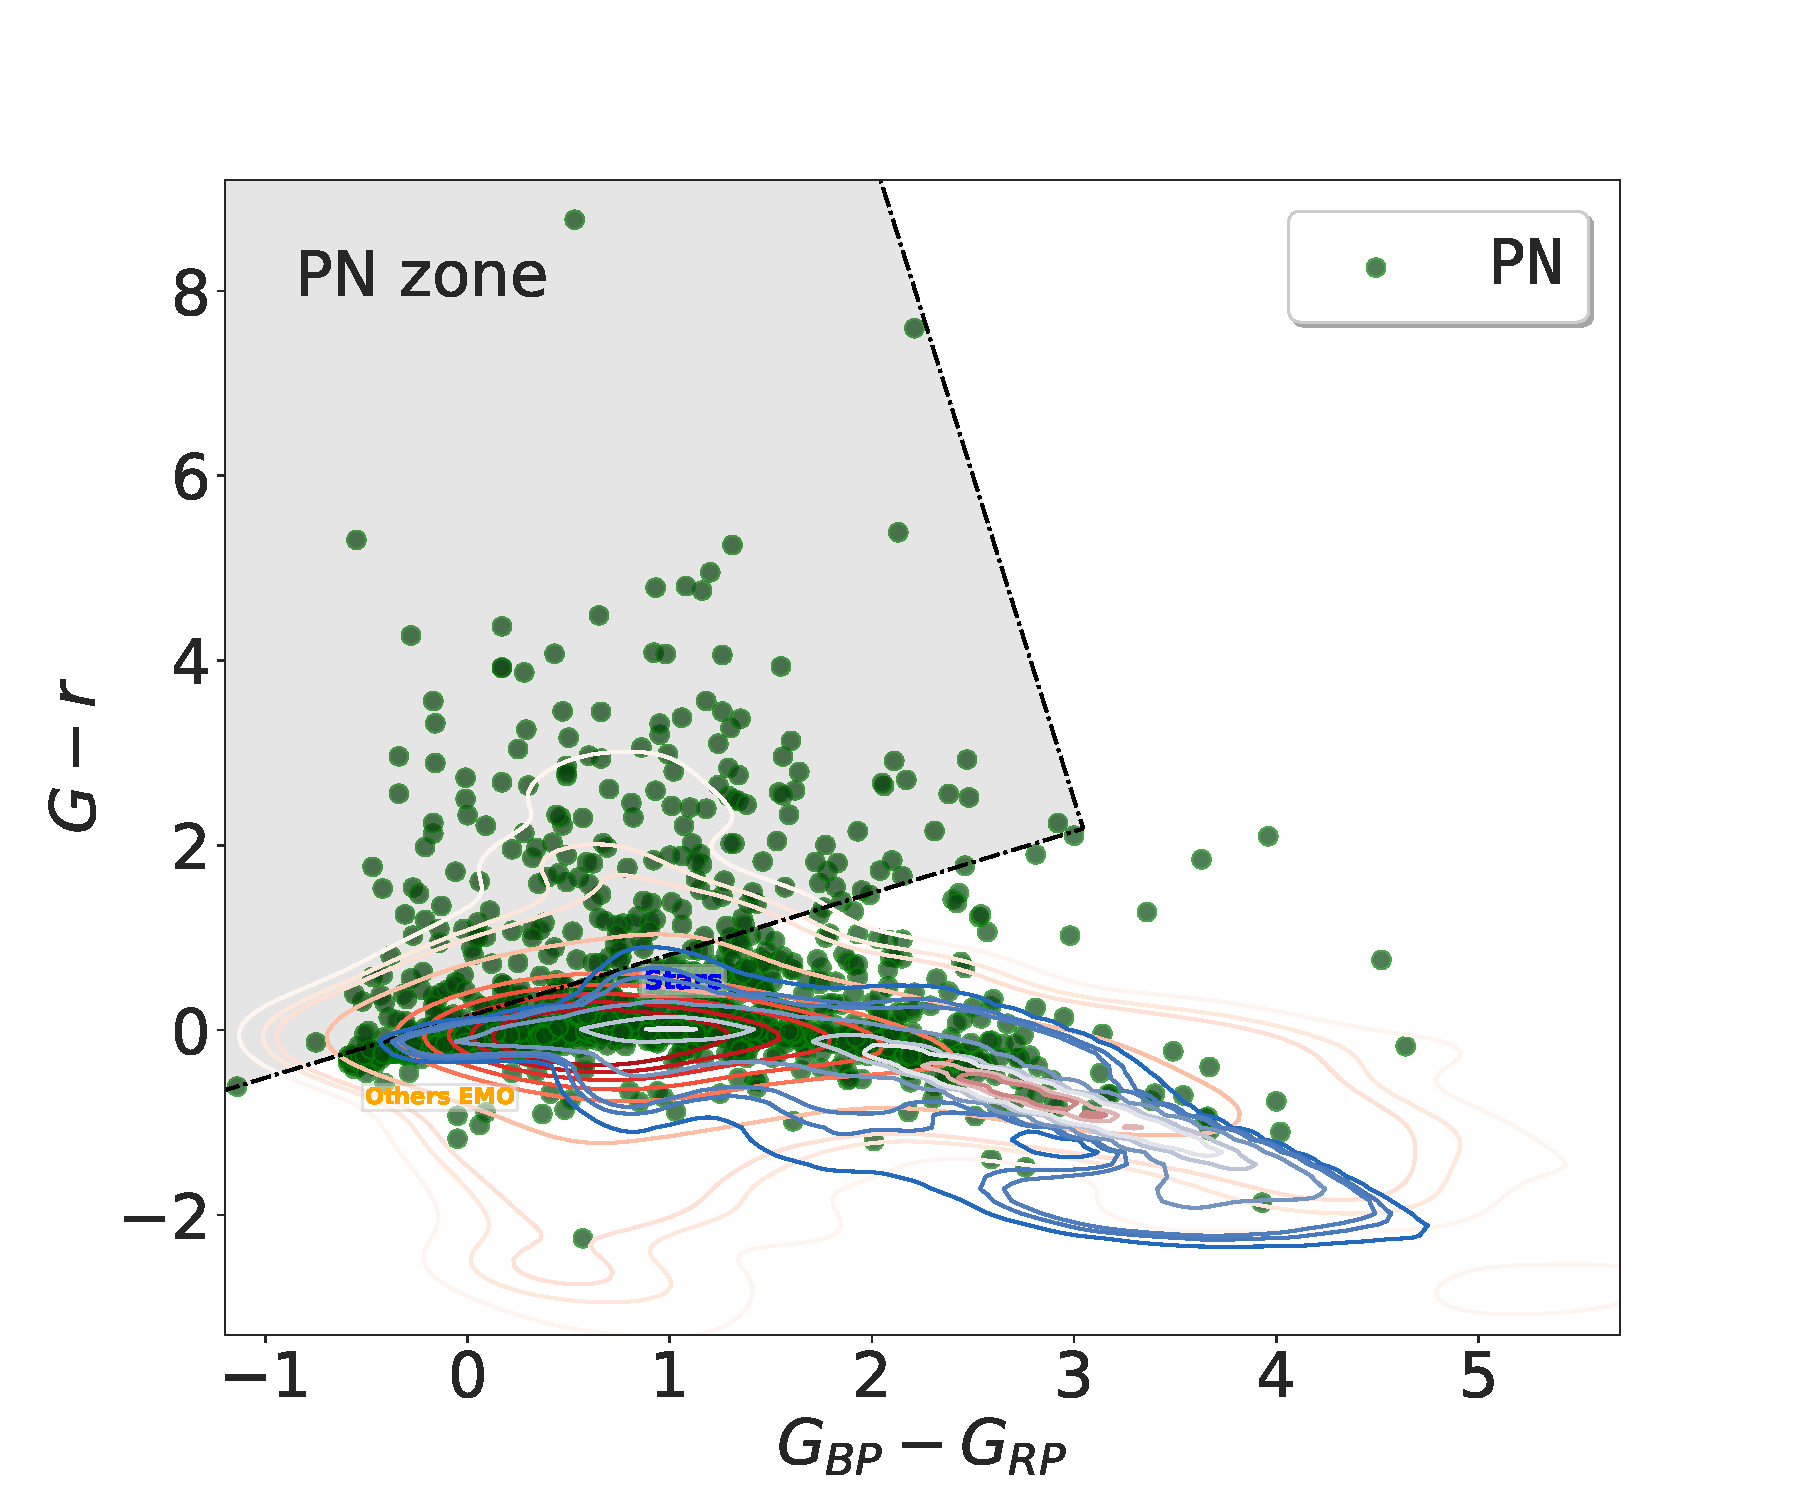
\includegraphics[width=0.9\linewidth]{../Figs/color-diagram-ps-gaiaEDR3.pdf}
  \caption{} 
  \label{fig:gaia-ps}
\end{figure}

All indicate that the PNe with strong \ha{} can be selected with this color criteria?.
Then, to see the possibility of using this color criterion to select these PNe, by
testing and using the emission line catalog from  \citet{Skoda:2020}. First, they
identify emission line objects from LAMOST  implementing a machine learning approach.
Then, they divided their final sample of emission line objects in tree subgroups. Those with \texttt{SIMBAD} coincidences, those that are listed by \citet{Hou:2016} and another list that are neither cross-matched with SIMBAD nor listed by  \citet{Hou:2016}. To texting the possibility to find for new PNe with the color criteria
explained above, we applied it directly in the new list, which present objects not reported
previously in the literature, which is a list with 1000 objects.

\begin{figure}
\centering
  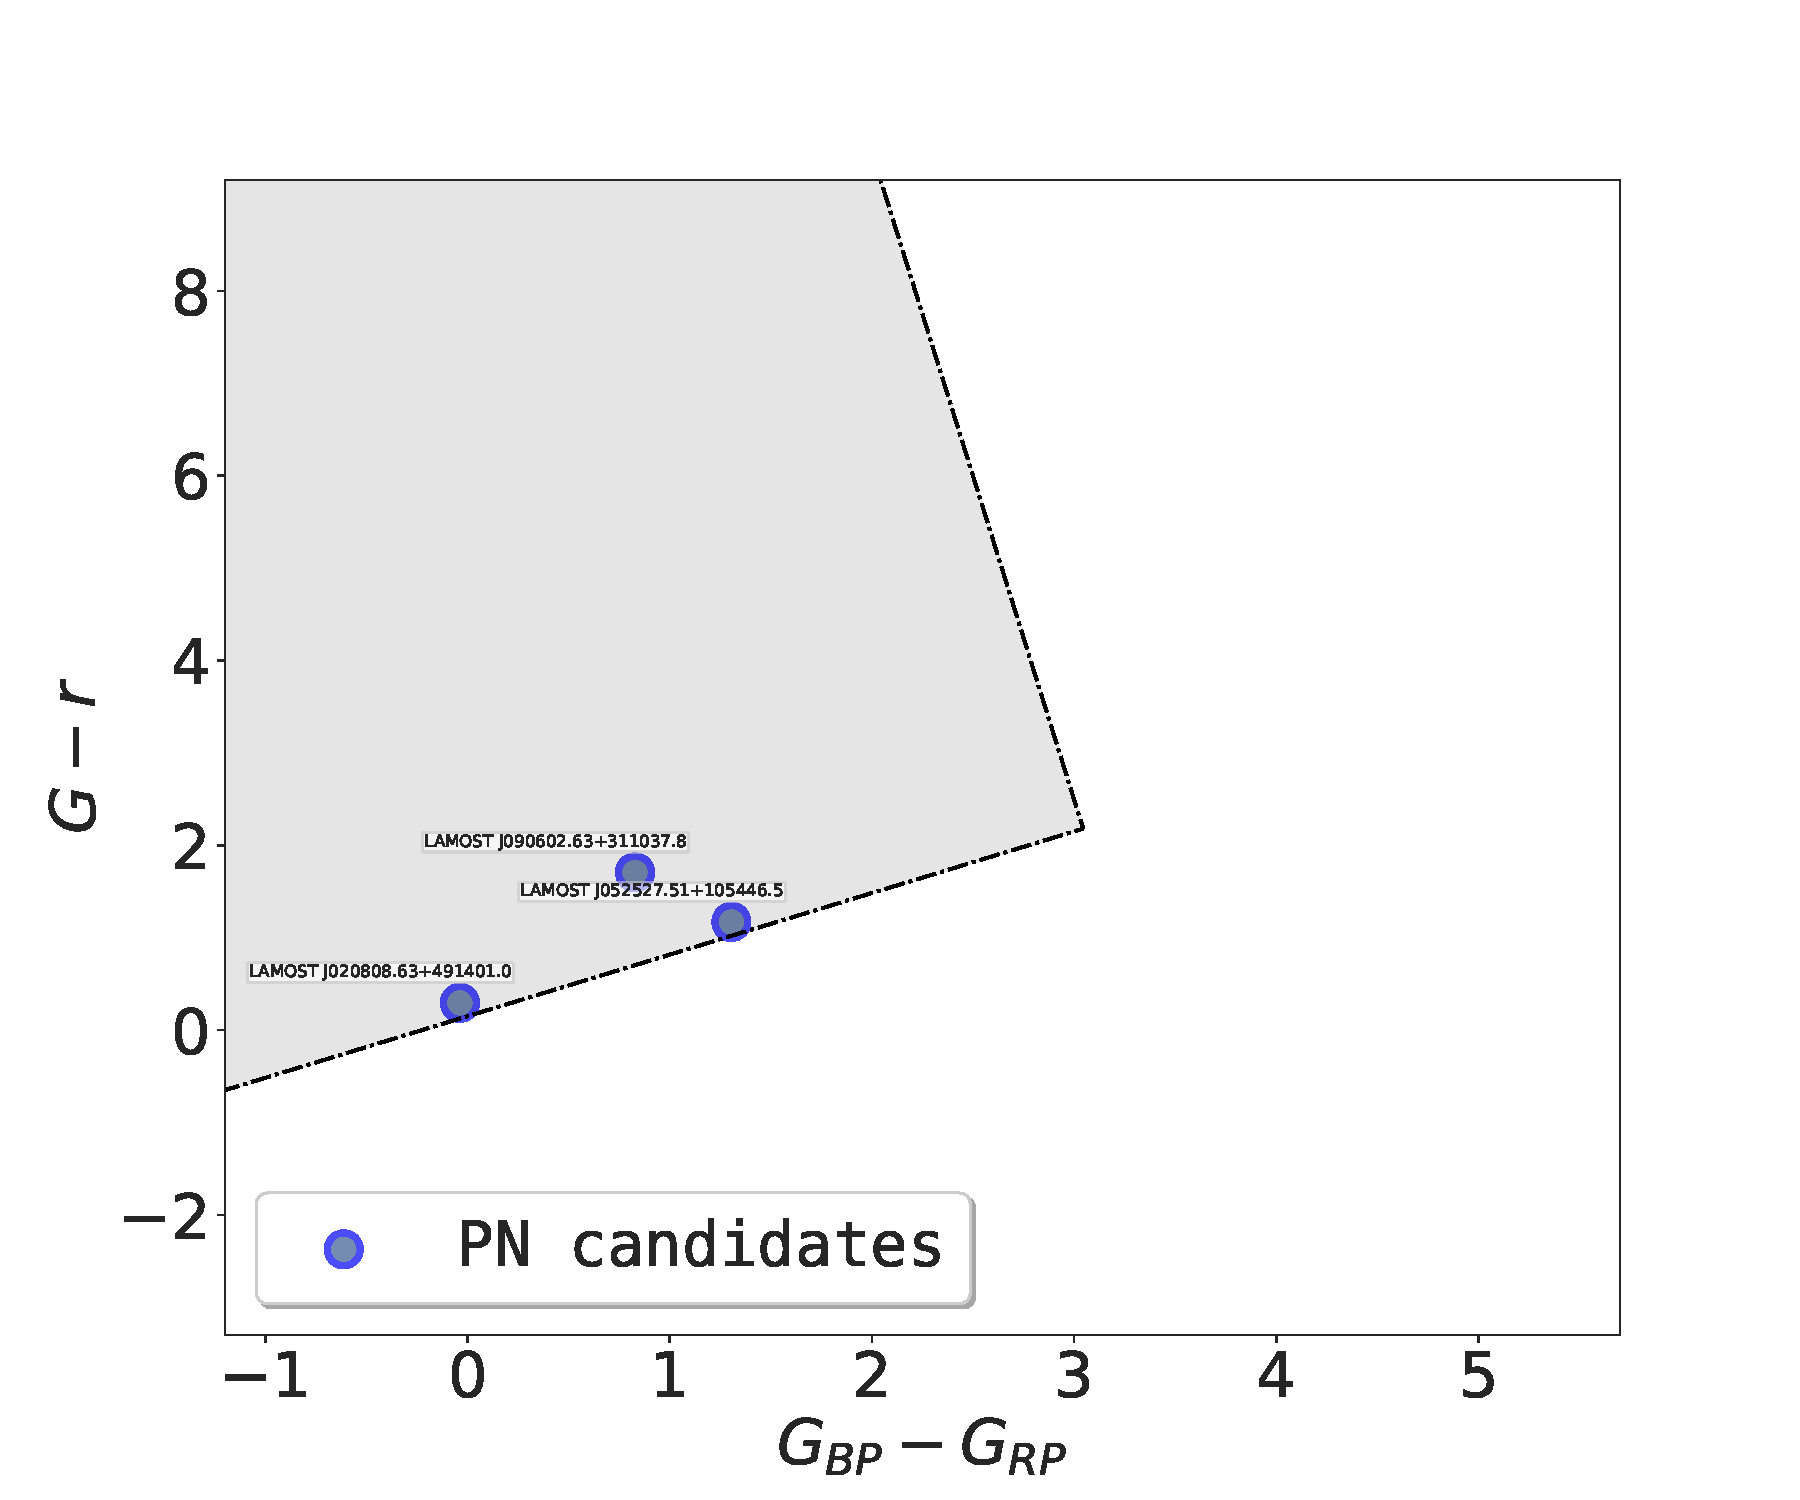
\includegraphics[width=0.9\linewidth]{../Figs/pn-candidates-gaiaDR3.pdf}
  \caption{} 
  \label{fig:gaia-ps-apply}
\end{figure}

Four objects met this  condition as is possible to see in the Fig~\ref{fig:gaia-ps-apply}.
We downloaded the low resolution spectra of these objects. 
Tree objects of them display strong \ha{}, but are not display the other emission lines topically
of PNe like [O III], He II, [S II], among other. But the three look likes as PNe.
Because, it displays He II emission lines, the Balmer ones, [O III], among others.
Fig~\ref{fig:spectra} the spectra of the new PN finding in the list of emission line of
\citet{Skoda:2020}. This PNe seem a very high ionization object, by eye is possible to see
that the He II emission line is as strong as the H$\beta$ line. Given the LAMOST spectra
are not calibrated in flux but they are flux relative, then I think that some ratio line can be calculated. Could be?

\begin{figure*}
\centering
  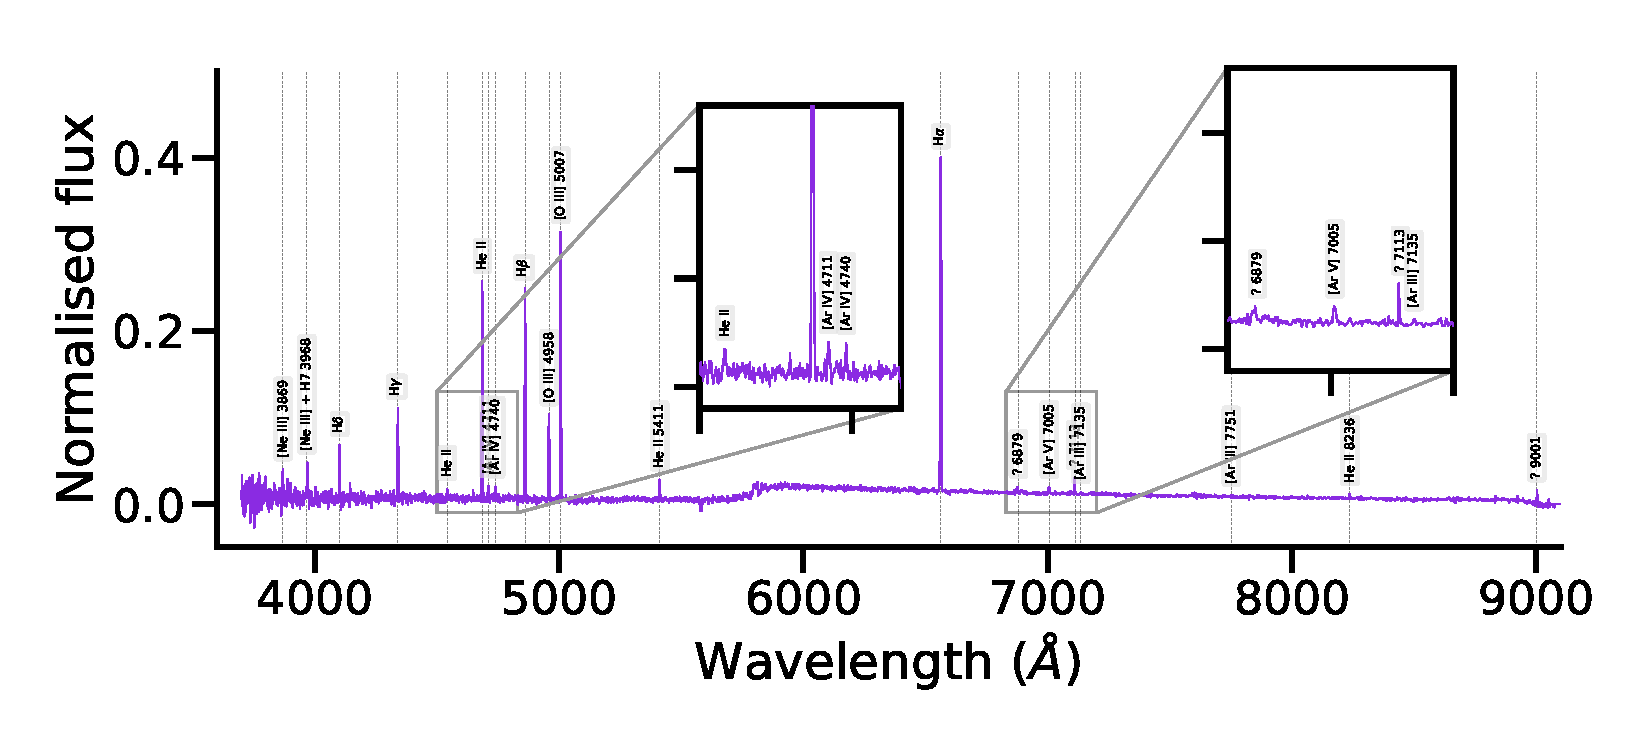
\includegraphics[width=0.9\linewidth]{../Spectra-lamostdr7/spec-56581-VB031N50V1_sp08-218.pdf}
  \caption{} 
  \label{fig:spectra}
\end{figure*}

The images of the PN called LAMOST J020808.63+491401.0 are shows in Fig~\ref{fig:image}.
\textit{Left panel} exhibits the PanSTARRS coloured
images \footnote{This RGB images were made by implementing
the python package \texttt{aplpy} \citep{aplpy:2019}}, which
was performed by combining the $g$, $r$ and $i$ filters in
the blue, green and red colour channels, respectively.
The image shows clearly a nebular component surrounding 
a central star. \textit{Right panel} shows the
WISE RGB image, with the filter W1, W2, and W4 in
the blue, green and red channels, respectively.  

\begin{figure*}
  \centering
  \begin{tabular}{l l}
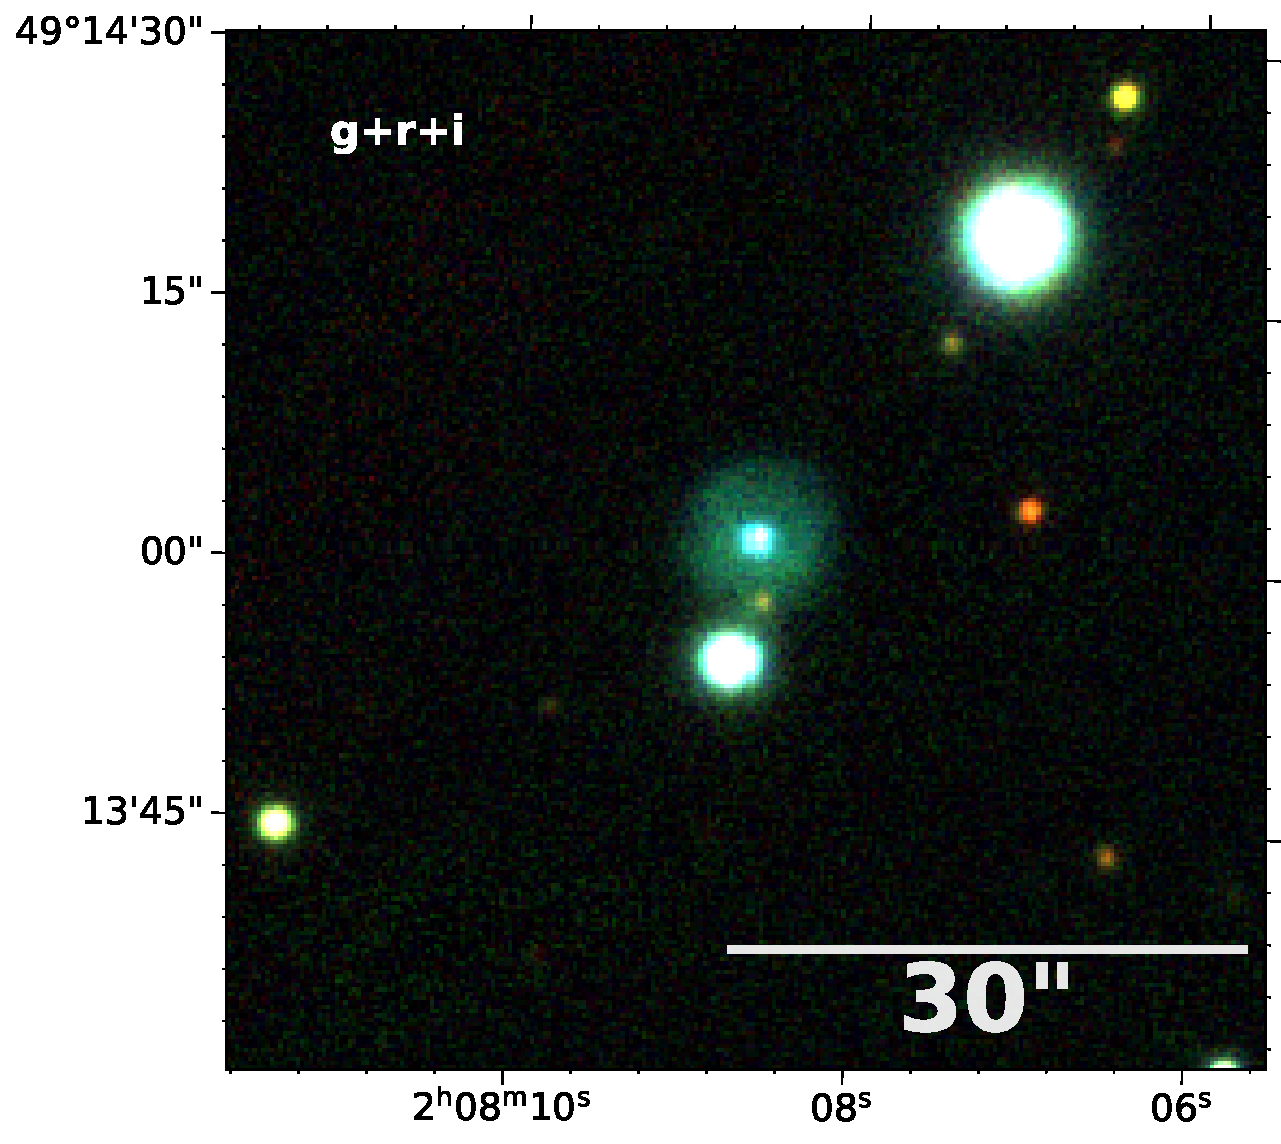
\includegraphics[width=0.5\linewidth]{../image-panstarr/cutout_rings_v3_skycell_2294_031_stk_i_unconv-irg-RGB.pdf}
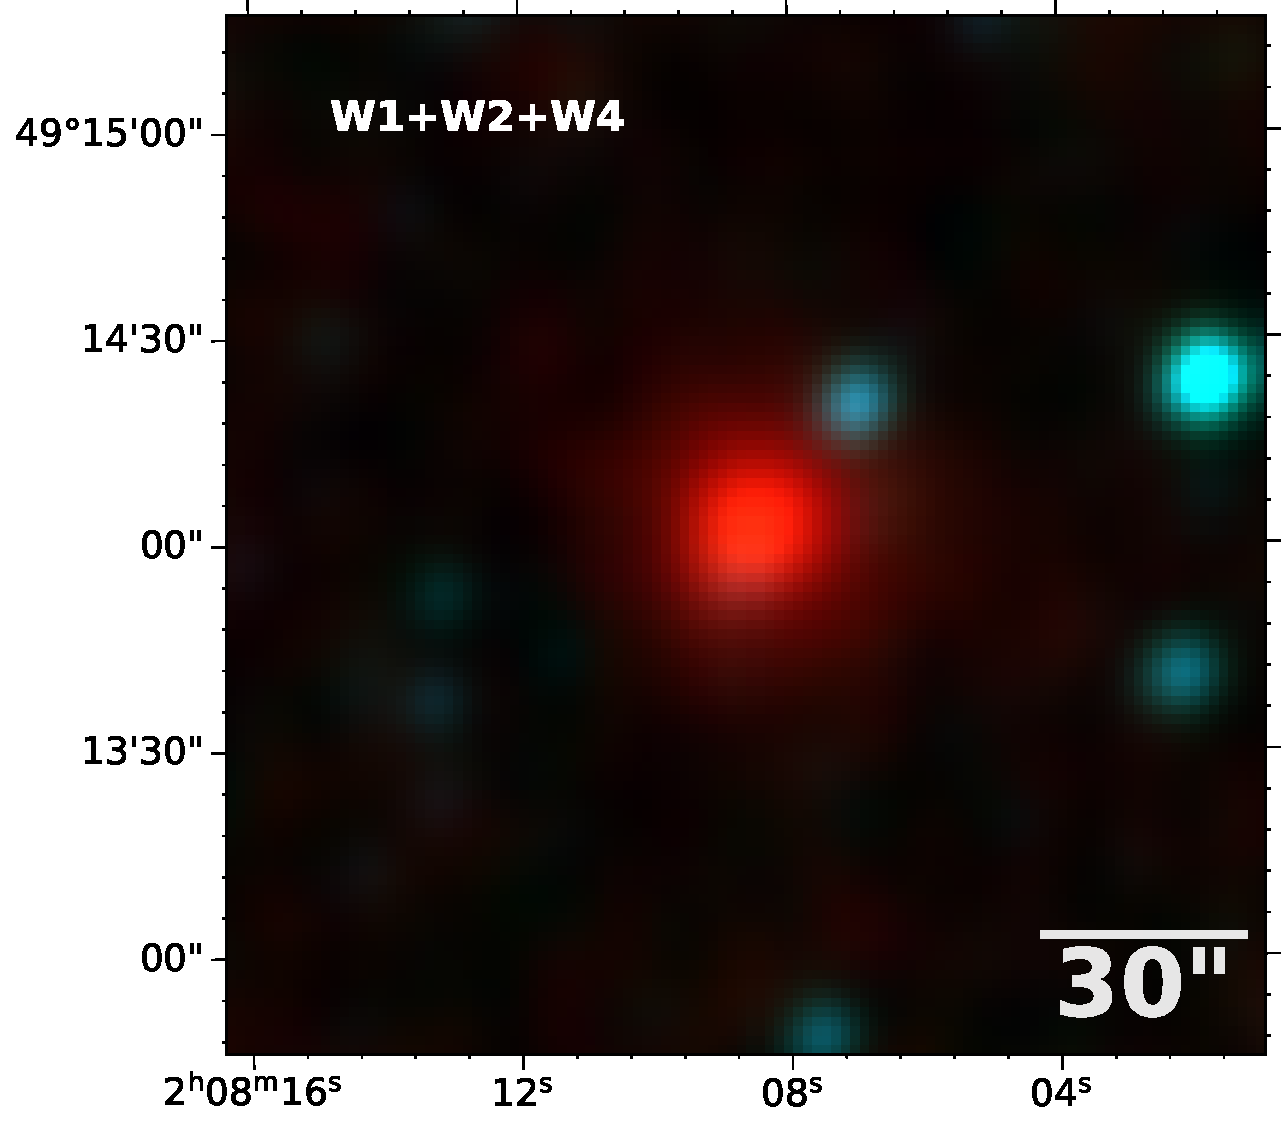
\includegraphics[width=0.5\linewidth]{../image-wise/w4_ra32_035994_dec49_233615-421-RGB.pdf}
\end{tabular}  
  \caption{} 
  \label{fig:image}
\end{figure*}


\section{Model}
\label{sec:model}

Despite the LAMOST spectra are not in physical flux unity, they have flux relative. This means it
is possible compare it with other spectra in physical units. For that, I think, it is pertinent to
compare the LAMOST spectra of our PN with models. Fig~\ref{fig:spectra-obs-model} shows a comparison between LAMOST spectra and a {\sc cloudy} modelled spectra from \citet{Gutierrez-Soto:2020}. Note that only is an example for illustrative intentions. This model was taken from a grid o models that reproduce spectra form the Galactic halo. For this, it don't exist a real matches between the two spectra. I will a performed a grid of PN models that better reproduce the LAMOST spectra of our candidate. However, almost all the line are reproduce with this model, that could be interesting, because the temperature effective of this model is 130$\times10^3$K, indicating a very high excitation object. Maybe, it will be good idea estimate ratio lines to confirm that! is it possible with this spectrum?

\begin{figure*}
\centering
  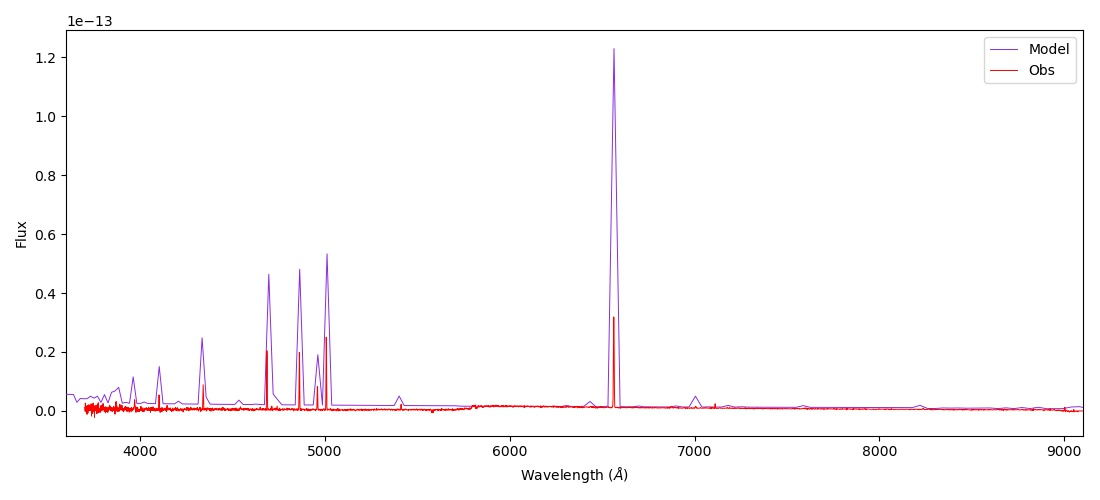
\includegraphics[width=0.89\linewidth]{../Spectra-lamostdr7/DdDm1_L4_T130_output_SED-E02-comparing-spectra}
  \caption{} 
  \label{fig:spectra-obs-model}
\end{figure*}

\section{Comparing with other PNe}
\label{sec:comp}

\newpage
\begin{figure*}
\centering
  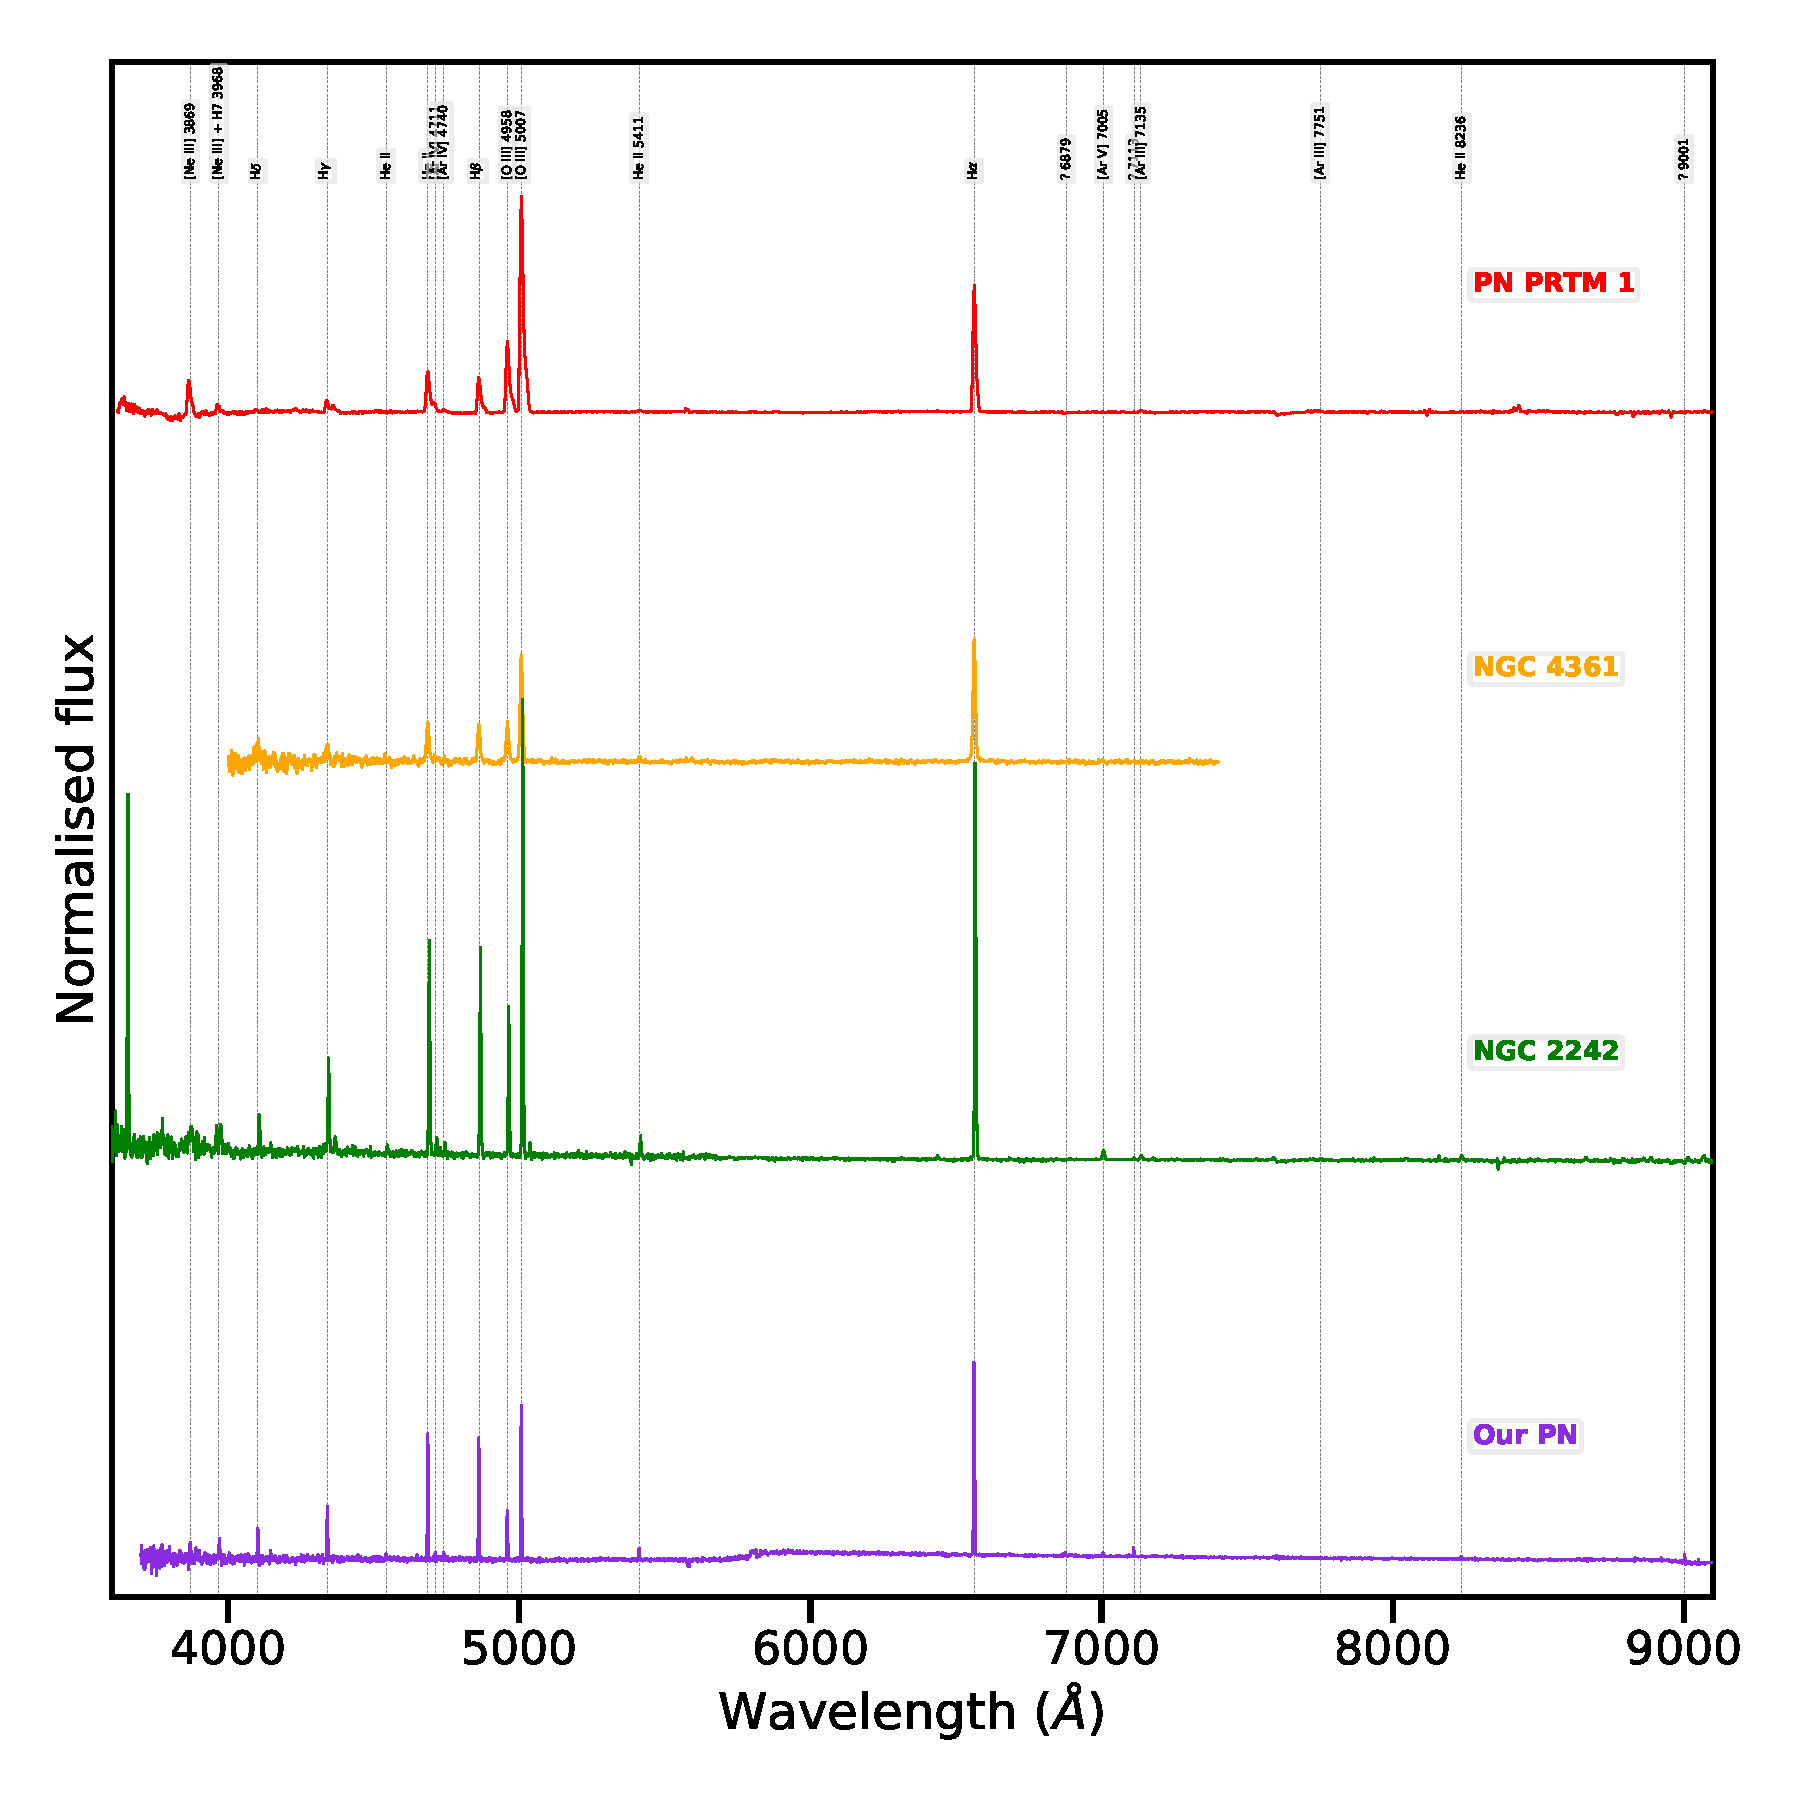
\includegraphics[width=0.8\linewidth]{../Figs/spectra-compare.pdf}
  \caption{Comparing the new PNe with other high halo palnetary nebulae...} 
  \label{fig:compare-spectra}
\end{figure*}

\bibliography{Ref-pne}

\end{document}

